\documentclass[a4paper,11pt,dvipdfmx]{jsarticle}

\usepackage{bm}
\usepackage[dvipdfmx]{graphicx}
\usepackage[dvipdfmx]{color}
\usepackage{ascmac}
\usepackage{amsmath}
\usepackage{amssymb}
\usepackage{siunitx}
\usepackage{otf}
\usepackage[dvipdfmx]{graphicx}
\pagestyle{plain}
\usepackage{float}
\usepackage[dvipdfmx]{hyperref}
\usepackage{pxjahyper}
\usepackage{here}
\usepackage{titlesec}
\titleformat*{\section}{\LARGE\bfseries}
\titleformat*{\subsection}{\normalsize\bfseries}
\usepackage{url}
\usepackage[table,xcdraw]{xcolor}
\hypersetup{% hyperrefオプションリスト
setpagesize=false,
 bookmarksnumbered=true,%
 bookmarksopen=true,%
 colorlinks=true,%
 linkcolor=blue,
 citecolor=blue,
}

\begin{document}
\renewcommand\thefootnote{\arabic{footnote})}
\subsection{非相対論の運動学}
微分散乱断面積は全て重心系で定義されるが、実際に測定が行われるのは実験室系である。以下では、実験室系における散乱の運動学及び実験室系と重心系の間の変換式について議論する。
\subsubsection{散乱の古典力学}
本節では散乱現象を弾性散乱と仮定する。今、以下のように実験室系において入射粒子と反跳粒子の2体の衝突を考える。

\begin{figure}[tbh]
\centering
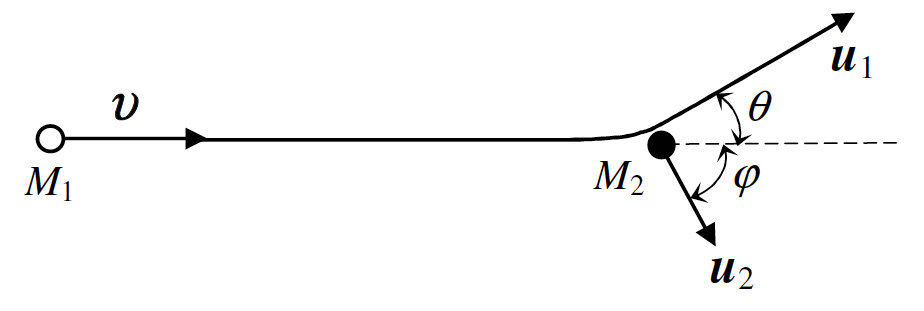
\includegraphics[width=8cm]{picture/nonrelativity/syototu.png}
\caption{実験室系における2体の衝突(\cite{ion}より引用し、一部改変)}
\label{fig:syototu}
\end{figure}

上の図\ref{fig:syototu}において入射粒子の質量を$M_{1}$、反跳粒子の質量を$M_{2}$とする。また、入射粒子の衝突前の速度を$\bm{v}$、衝突後の速度を$\bm{u_{1}}$、反跳粒子の速度を$\bm{u_{2}}$とする。この時、運動量保存とエネルギー保存を考えると、
\begin{equation}
\frac{1}{2}M_{1}v^{2} = \frac{1}{2}M_{1}u_{1}^{2} + \frac{1}{2}M_{2}u_{2}^{2}
\end{equation}
\begin{equation}
M_{1}v = M_{1}u_{1}\cos\theta+M_{2}u_{2}\cos\varphi
\end{equation}
\begin{equation}
0 = M_{1}u_{1}\sin\theta-M_{2}u_{2}\sin\varphi
\end{equation}
が成り立つ。3つの式に対して、4つの未知数$u_{1}$、$u_{2}$、$\theta$、$\varphi$があるので、連立することで以下の関係式が得られる。
\begin{equation}\label{eq:kakudo}
\tan\theta = \frac{M_{2}\sin2\varphi}{M_{1}-M_{2}\cos2\varphi}   
\end{equation}
\begin{equation}
E = \frac{1}{2}M_{1}u_{1}^{2} = \left(\frac{M_{1}\cos\theta + \sqrt{M_{2}^{2} - M_{1}^{2}\sin^2\theta}}{M_{1}+M_{2}}\right)^{2}E_{0}
\label{eq:energy}
\end{equation}
\begin{equation}\label{eq:recoil}
T = \frac{1}{2}M_{2}u_{2}^{2} = \frac{4M_{1}M_{2}}{\left(M_{1}+M_{2}\right)^{2}}E_{0}\cos^2\varphi
\end{equation}
ただし、$E_{0} = \frac{1}{2}M_{1}v^{2}$である。ここで、$E$は散乱陽子のエネルギーである。
また、(\ref{eq:kakudo})~(\ref{eq:recoil})式を $A = \frac{M_{2}}{M_{1}}$を用いて書き直すと、以下のようになる。
\begin{equation}\label{eq:kakudokai}
\tan\theta = \frac{A\sin2\varphi}{1 - A\cos2\varphi}   
\end{equation}
\begin{equation}
E  = \left(\frac{\cos\theta + \sqrt{\cos^2\theta + A^{2} -1}}{A + 1}\right)^{2}E_{0}
\label{eq:energykai}
\end{equation}
\begin{equation}\label{eq:recoilkai}
T = \frac{4A}{\left(A + 1\right)^{2}}E_{0}\cos^2\varphi
\end{equation}

\eqref{eq:energykai}、\eqref{eq:recoilkai}をグラフにすると、図\ref{fig:scaene}、図\ref{fig:recoil}のようになる。ただし、$E_{0}=$\;3\;MeVである。

\begin{figure}[bhtp]
  \begin{minipage}{0.5\hsize}
    \begin{center}
      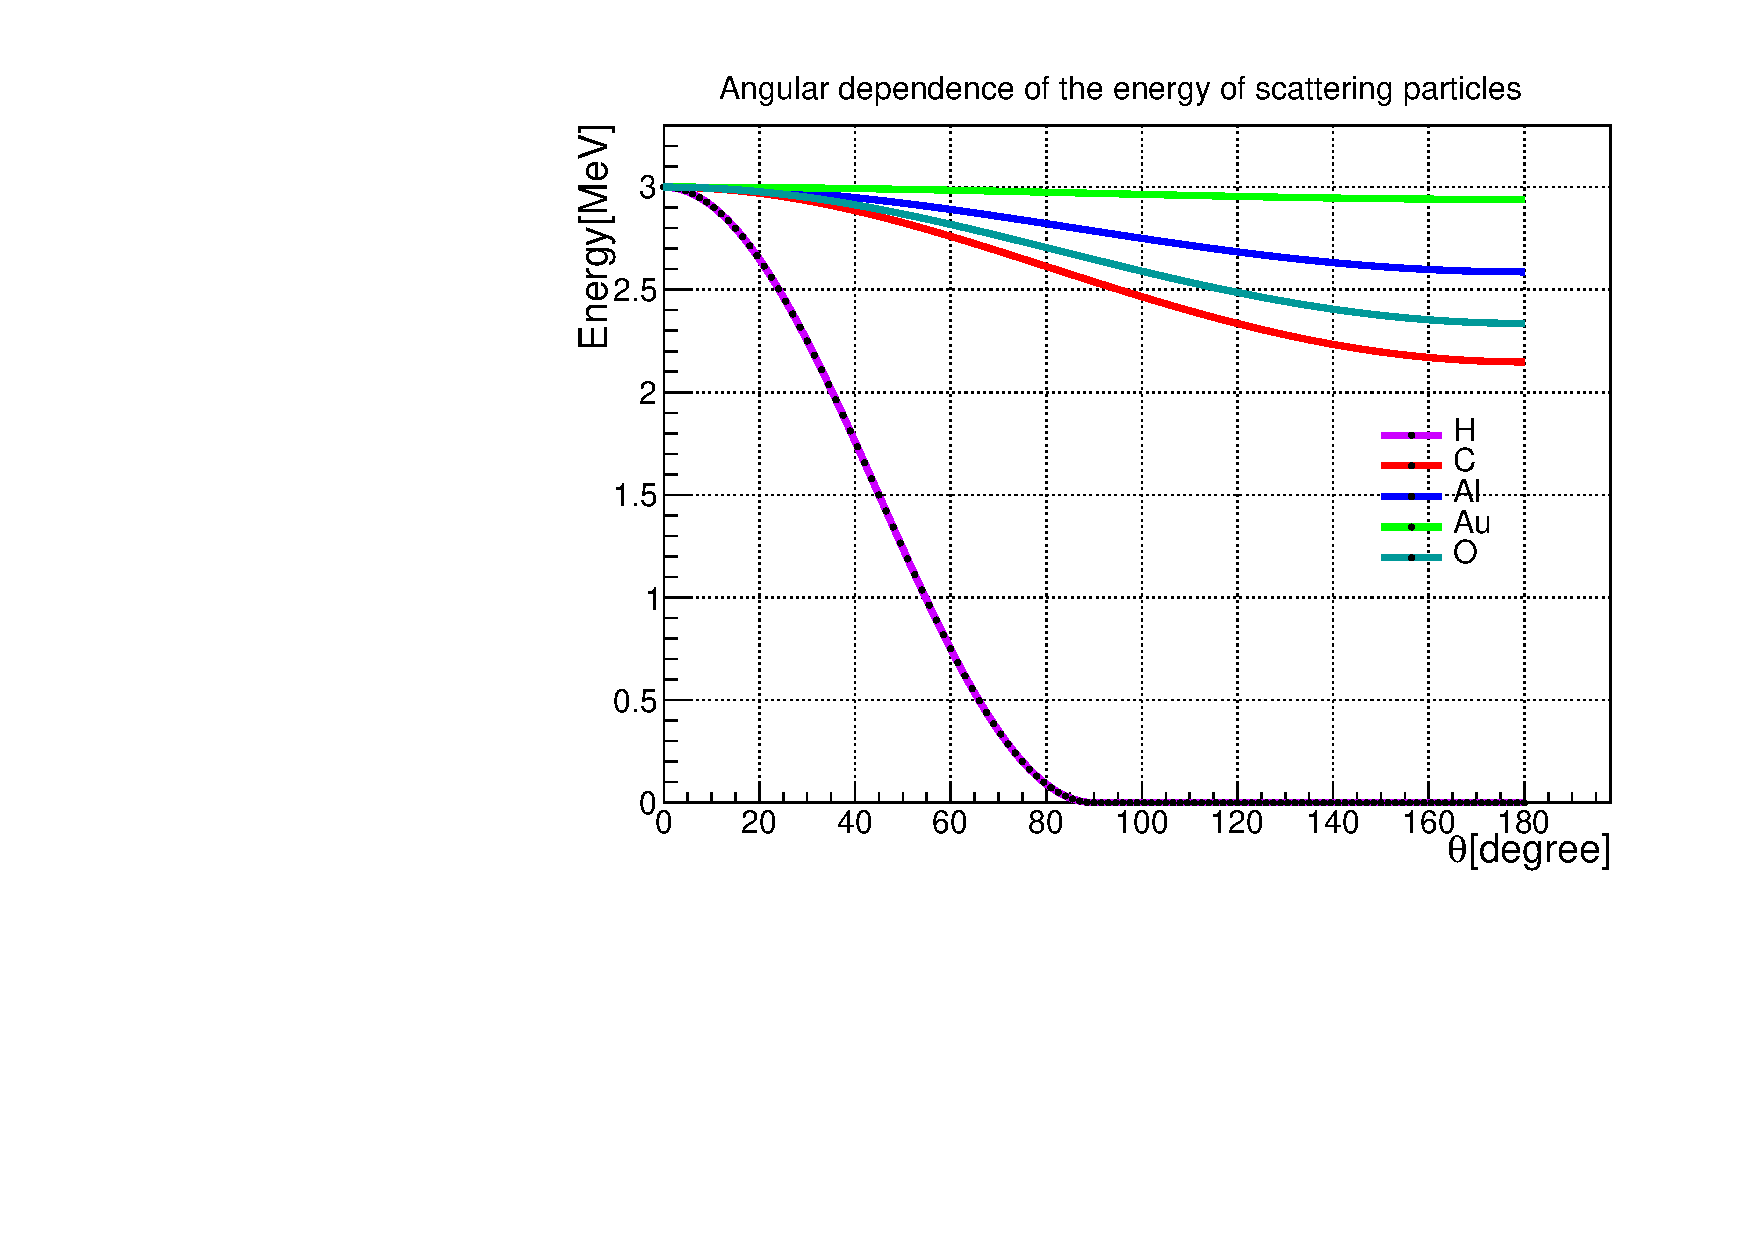
\includegraphics[width=73mm]{picture/nonrelativity/newsca.pdf}
    \end{center}
    \caption{散乱陽子のエネルギー}
    \label{fig:scaene}
  \end{minipage}
  \begin{minipage}{0.5\hsize}
    \begin{center}
      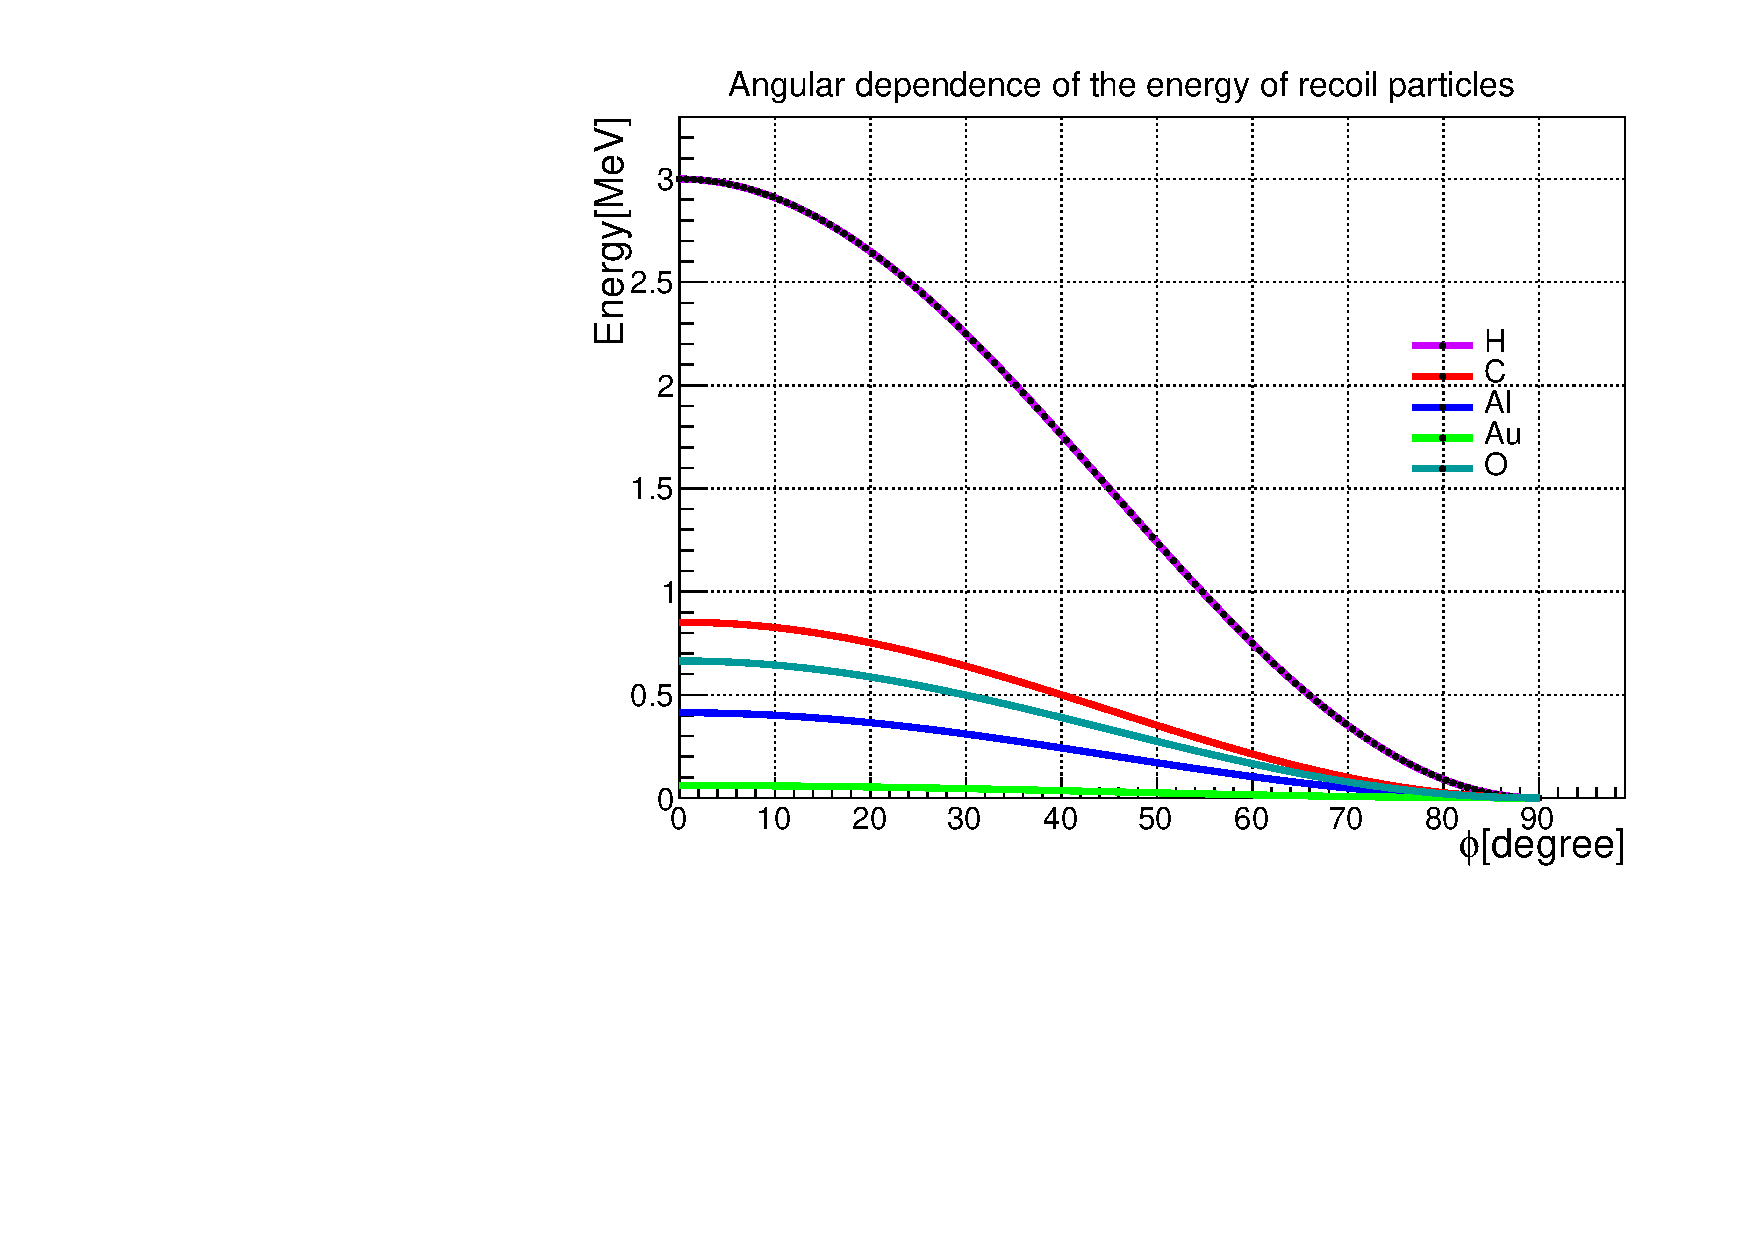
\includegraphics[width=73mm]{picture/nonrelativity/recoil.pdf}
    \end{center}
    \caption{反跳粒子のエネルギー}
    \label{fig:recoil} 
  \end{minipage}
\end{figure}
\newpage
\subsubsection{p-p散乱のopening angle}\label{opening}
次にp-p散乱(陽子-陽子散乱)のopening angleについて考える。

p-p散乱の場合$A = 1$なので、(\ref{eq:kakudokai})式から以下の式が導かれる。
\begin{equation}\label{eq:ten}
\tan\theta = \frac{\sin2\varphi}{1 - \cos2\varphi} =\frac{1}{\tan\varphi}
\end{equation}
(\ref{eq:ten})の方程式を解くことで、
\begin{equation}
\theta + \varphi = 90^{\circ}
\end{equation}
となるので、p-p散乱のopening angleは $90^{\circ}$になる。

\subsubsection{実験室系、重心系間の変換式}
前述の通り微分散乱断面積は重心系で定義されるが、実際には実験室系で測定されるので実験室系における物理量を重心系に変換する必要が出てくる。

後述する相対論の影響がないとすると、実験室系での散乱角$\theta$と重心系での散乱角$\theta_{cm}$の間に成り立つ関係式は、
\begin{equation}
    \tan\theta = \frac{\sin\theta_{cm}}{\cos\theta_{cm}+\frac{1}{n}}\label{eq:henkan1}
\end{equation}
となる\cite{kyodai}。ただし、$n=m_{2}/m_{1}$である。

p-p散乱の場合、$n=1$なので
\begin{equation}
    \theta=\frac{\theta_{cm}}{2}
\end{equation}
が成り立つ。

また、実験室系と重心系における微分散乱断面積をそれぞれ$\left(\frac{d\sigma}{d\Omega}\right)_\text{lab}$,$\left(\frac{d\sigma}{d\Omega}\right)_\text{cm}$とすると、これらの間の関係式は
\begin{equation}
    \left(\frac{d\sigma}{d\Omega}\right)_\text{cm} = \frac{1+\frac{\cos\theta_{cm}}{n}}{\left(1+\frac{2}{n}\cos\theta_{cm}+\frac{1}{n^2}\right)^{\frac{3}{2}}}\left(\frac{d\sigma}{d\Omega}\right)_\text{lab}\label{eq:henkan2}
\end{equation}
で表される\cite{kyodai}。


\end{document}